\documentclass[sigplan, review]{acmart}

\usepackage{booktabs,amsmath,capt-of,lipsum} % For formal tables


% Copyright
%\setcopyright{none}
%\setcopyright{acmcopyright}
%\setcopyright{acmlicensed}
\setcopyright{rightsretained}
%\setcopyright{usgov}
%\setcopyright{usgovmixed}
%\setcopyright{cagov}
%\setcopyright{cagovmixed}


% DOI
% \acmDOI{10.475/123_4}

% % ISBN
% \acmISBN{123-4567-24-567/08/06}

%Conference
\acmConference[Compiler Construction]{CSCI 4555/5525 and ECEN 4553/5523}{Fall 2017}{Boulder, CO USA}
\acmYear{2017}
\copyrightyear{2017}

% \acmPrice{15.00}

%\acmBadgeL[http://ctuning.org/ae/ppopp2016.html]{ae-logo}
%\acmBadgeR[http://ctuning.org/ae/ppopp2016.html]{ae-logo}


\begin{document}
\title{Compiling python to a side-channel protected binary}

\author{Sergey Frolov}
\affiliation{%
  \institution{University of Colorado}
  \city{Boulder} 
  \state{CO}
  \country{USA}
}
\email{sergey.frolov@colorado.edu}

\author{Albert Dayn}
\affiliation{%
  \institution{University of Colorado}
  \city{Boulder} 
  \state{CO}
  \country{USA}
}
\email{albert.dayn@colorado.edu}

% The default list of authors is too long for headers.
% \renewcommand{\shortauthors}{B. Trovato et al.}


\begin{abstract}
There are numerous side-channel based attacks on protections, guaranteed by Intel SGX trusted execution. Prior research has shown that side-channels may enable a local attacker to extract information from the secure enclave. We address issues with cache, timing, and branch shadowing through a combination of known and brand new techniques to compile Python to a protected binary. We show that proposed protections efficiently eliminate side-channels.
\end{abstract}

%
% The code below should be generated by the tool at
% http://dl.acm.org/ccs.cfm
% Please copy and paste the code instead of the example below. 
%
\begin{CCSXML}
<ccs2012>
<concept>
<concept_id>10011007.10011006.10011041</concept_id>
<concept_desc>Software and its engineering~Compilers</concept_desc>
<concept_significance>500</concept_significance>
</concept>
<concept>
<concept_id>10002978.10003022</concept_id>
<concept_desc>Security and privacy~Software ansd application security</concept_desc>
<concept_significance>300</concept_significance>
</concept>
</ccs2012>
\end{CCSXML}

\ccsdesc[500]{Software and its engineering~Compilers}
\ccsdesc[300]{Security and privacy~Software and application security}


\keywords{Compilers, Intel SGX, side-channels, secure code generation}

\maketitle

\section{Introduction}
Intel Software Guard Extensions (SGX) enables trusted execution with a new set of CPU instructions and platform enhancements, allowing a dramatic increase privacy, security and sometimes scalability of applications, when used correctly. Specifically, it allows applications to protect portions of code and data (an “enclave”) from manipulation, even from a potentially compromised OS. The enclave is protected from disclosure, as data is always encrypted in RAM. Intel SGX also allows users to easily perform operations that are either very computationally expensive in software-only solutions (such as Private Information Recovery~\cite{signalprivaterecovery} and mutually distrusted computation on shared data), or simply impossible (remote attestation, which allows client to prove to a remote entity the integrity of software running inside of enclave).\\
However, side-channels have proved to be a very serious limitation of SGX. Several attacks on SGX are known, including timing and cache-based side-channels, as well as branch shadowing. While some algorithms may be immune to those attacks due to inherent lack of any branching, there are cases in which side-channels would work extremely effective, e.g. allowing to extract full RSA private key~\cite{schwarz2017malware} in an automated attack in under 5 minutes.\\
Whenever application developers are accept the complexities of using SGX, they rely on its protections and assumptions heavily, and when those assumptions are broken even in a minor way, the security of whole application may be compromised. For this reason, it is crucial to find effective means to defeat those attacks in a manner, without making the solution too cumbersome to potential users. Specifically, users need to be able to write idiomatic code and ensure it compiles to a constant time binary.
This paper describes known SGX side-channels, and presents effective defences. Description of proposed defences’ design is followed by performance evaluation, which shows the effectiveness of our suggested timing side-channel protections.

\section{Background}
Intel SGX allows applications to put portions of code and data into a so-called “secure enclave”, and protect it from manipulation from any local attacker, including a malicious or compromised operating system. As everything in this “secure enclave” is encrypted, Intel SGX also effectively protects data from disclosure. Such strong protections may prove challenging to ensure, however, since local attackers have various tools at their disposal to mount attacks. Since the secure enclave shares the processor with the attacker, information may leak through side-channels such as timing, processor cache, Branch Target Buffer, and other shared physical resources. Even though there are usually no direct ways to probe those resources, the attacker may do this indirectly. Also note that it is within a local attacker’s power to interrupt the secure enclave’s execution at will, which makes attacks easier to perform in practice.\\
A proper understanding of our side-channel protections requires knowledge of corresponding attacks, and we proceed to describe previously introduced exploitation techniques in this section. Generally, attacks are executed right after interrupting enclave and attempting to infer something about what just happened inside of an enclave. For the attacks that we protect against, the adversary wants to use a particular side-channel to determine which branch (at the assembly level) was taken.\\
\textbf{Timing attack.}\cite{kocher1996timing} A timing attack is relatively easy and intuitive. Suppose we have 2 or more branches, which take different amount of time to execute. A local attacker may measure time spent on execution and derive which branch was taken, allowing them to infer the value of the tested conditional.\\
\textbf{Cache attack.}\cite{osvik2006cache} To carry out this attack, the adversary fills the cache with random data, then lets the enclave continue execution. After secure enclave executes the target branch, attacker would interrupt the enclave. Now, the attacker is able to probe the cache, by accessing the same random data and measuring the time it took to fetch it. Form this, they can determine which cache lines were evicted by the enclave. Since the cache line used depends on the memory address, which varies based on the variables used in different branches, the attacker may infer which branch was taken in the enclave.\\
\textbf{Branch shadowing attack.}\cite{lee2016inferring} This attack allows local attacker to determine whether an enclave branch at a certain address, e.g., \texttt{0x0000422410}, was taken, a by crafting “shadowing” out-of-enclave branch at e.g. \texttt{0xffff422410}, which shares lower 31 bits of the address. Since only those last bits are used to locate an entry in Branch Target Buffer table, enclave branch will collide with out-of-enclave branch. After attacker executes the out-of-enclave branch, they’d be able to measure elapsed cycles and checking LBR table, see whether the out-of-enclave was mispredicted, and learn whether corresponding branch was taken in enclave.
Attack on memory access patterns. The operating system has access to encrypted RAM, and so may be able to derive memory access patterns from page faults. Suppose the enclave accesses certain index of an array, and will have to go to memory for this. Despite the fact that RAM, used by enclave, is encrypted, operating system still has access to memory accesses and page faults, and may be able to infer the index of an array, enclave tries to access. This will be problematic, since index of an array may be precisely the data application wants to hide, for example this was the case in private contact discovery for Signal messenger~\cite{signalprivaterecovery}. This attack is not covered in this project and left for future work.

\section{Implementation}
Definitions: \textit{conditional jump instruction} refers to instructions which may or may not perform a jump to a static address (e.g. \texttt{jne LOOP}). \textit{indirect jump instruction} refers to instructions that always jump to a dynamic address (e.g. \texttt{jmp *\%ebx}). \textit{unconditional jump instruction} refers to instructions that always jump to a static address (e.g. \texttt{jmp LOOP}).

\begin{align*}
program         \ ::=&\ ef\!f\!ectStmts\\\\
ef\!f\!ectStmts \ ::=&\ ef\!f\!ectStmt\ ef\!f\!ectStmts \\
                    |&\ \epsilon \\\\
ef\!f\!ectStmt  \ ::=&\ \text{``input''}\ \text{``(''}\ \text{``)''}\\
                    |&\ \text{``print''}\ expr\\
                    |&\ simpleStmt\\\\
simpleStmts     \ ::=&\ simpleStmt\ simpleStmts \\
                    |&\ \epsilon \\\\
simpleStmt      \ ::=&\ \text{``if''}\ expr\ \text{``:''}\\
                     &\qquad suite\\
                     &\ \text{``else''}\ \text{``:''}\\
                     &\qquad suite\\
                    |&\ \text{``if''}\ expr\ \text{``:''}\\
                     &\qquad suite\\
                    |&\ \text{``while''}\ expr\ \text{``:''}\\\
                     &\qquad suite\\
                    |&\ x\ \text{``=''}\ expr\\\\
suite           \ ::=&\ \text{INDENT}\ simpleStmts\ \text{DEDENT}\\\\
expr            \ ::=&\ expr\ \text{``if''}\ expr\ \text{``else''}\ expr\\
                    |&\ expr\ \text{``+''}\ expr\\
                    |&\ \text{``not''}\ expr\\
                    |&\ \text{``-''}\ expr\\
                    |&\ n\\
                    |&\ x
\end{align*}

\begingroup\vspace*{-\baselineskip}
\captionof{figure}{The subset of Python implemented in our prototype compiler. Notice the distinction between simple and effect statements, and the type used in a suite.}
\vspace*{\baselineskip}\endgroup
% \lipsum*[2]

We have implemented a constant time compiler which hardens a subset of Python against timing, cache, and branch shadowing side-channels. The specific language fragment is defined below. Notice that \textit{effect\_statements} (statements which perform observable side effects other than memory access) are allowed only outside of \texttt{if} statements, otherwise the semantics of the language would change as a result of our transformations. We feel this is an acceptable trade off for constant time compilation, as conditional side effecting statements expose an unsafe side-channel themselves.\\

Our side-channel protections consist of three separate phases, which build on the Zigzagger \cite{lee2016inferring} mitigation. Zigzagger is a method of compiling conditional control flow using only conditional move and indirect jump instructions, meaning no branch prediction is done by the cpu, preventing the leakage of branch history outside of SGX through branch shadowing. The first protection we explored used this method unaltered to compile \texttt{while} loops to an assembly equivalent without using leaky conditional jump instructions to protect while loops against branch shadowing. The second protection improves upon Zigzagger by transforming \texttt{if} statements into an assembly equivalent with no conditional or indirect jump instructions to protect against timing attacks. The third protection prevents memory from being conditionally read in cmov instructions to protect against cache side-channels. Authors of Zigzagger mention that “measuring branch prediction/misprediction penalties based on timing is too inaccurate to distinguish fine-grained control-flow changes”, but we have decided to close this side-channel none the less, as viable attacks have already been presented and proved viable, which are referenced in Related Work.\\
\subsection{Branch Shadowing defense}
Using the Zigzagger mitigation, we perform transformation on while loops, as depicted on Figure \ref{fig:while_zigzagger}.

\begin{figure}[bhp]
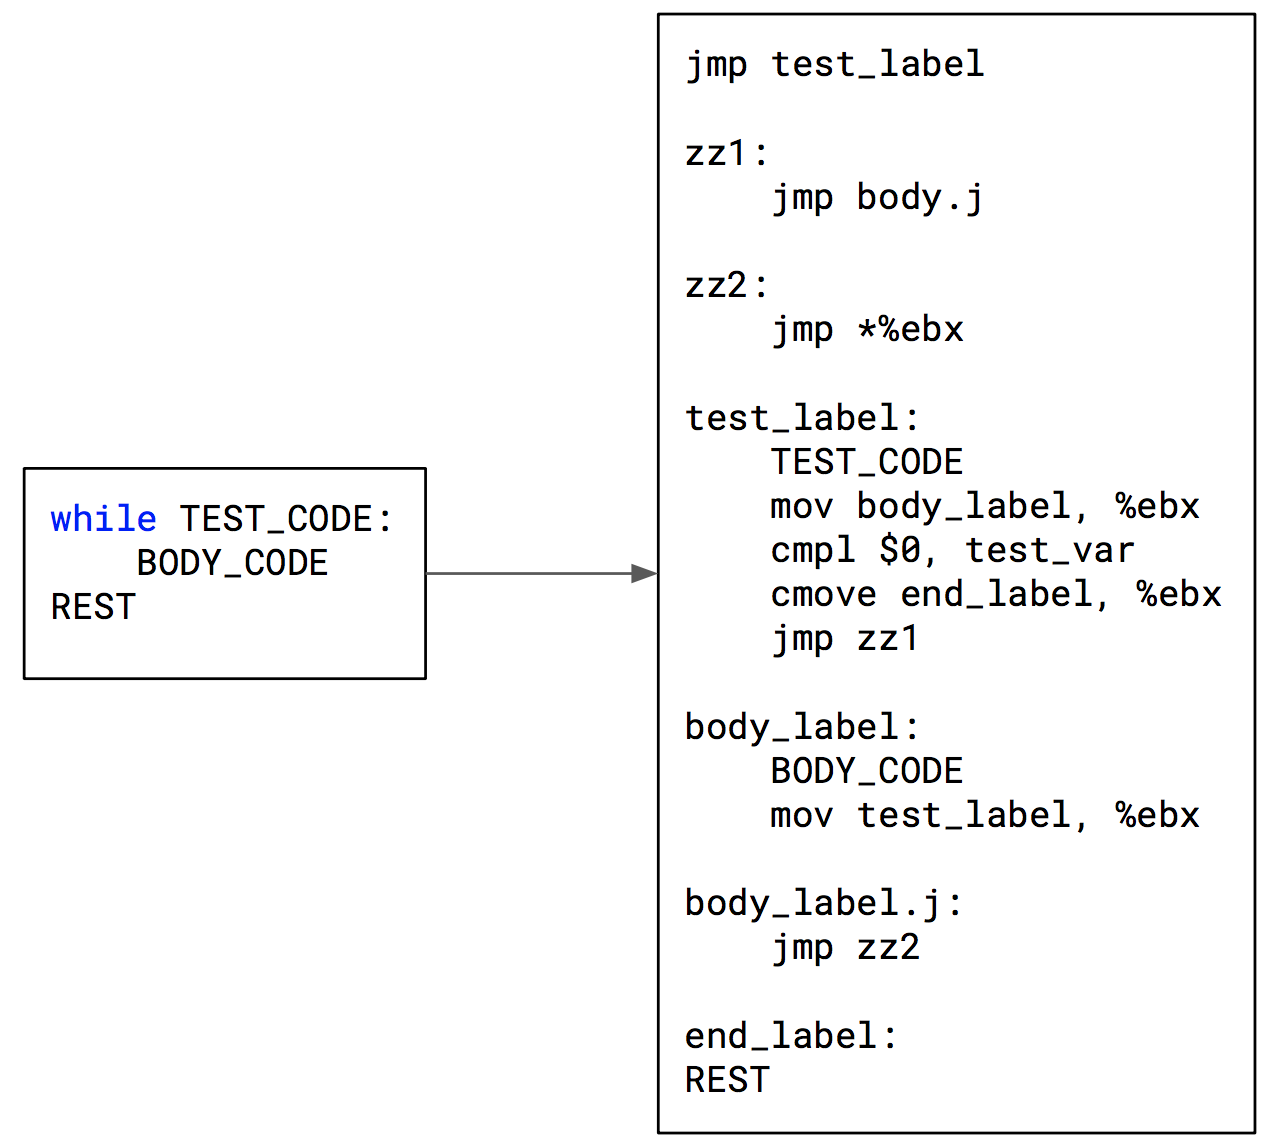
\includegraphics[width=\columnwidth]{./while_zigzagger.png}
\caption{The transformation applied by our compiler on while loops, based on the mitigation on if statements in Lee, Sangho, et al.}
\label{fig:while_zigzagger}
\end{figure}

We reserve the \texttt{ebx} register to store the address we want the Zigzagger trampoline to jump to next (instead of \texttt{r15} as used in Lee, Sangho, et al.~\cite{lee2016inferring}). Execution begins by jumping over the inserted Zigzagger trampoline and into the test code. Once the test is performed, we initialize \texttt{ebx} to the body code, assuming it will be executed. If the result of the test was \texttt{false}, the end label is instead moved into \texttt{ebx}. We then jump to the start of the trampoline, and, as described in Zigzagger, we go through a series of unconditional jumps until we reach the final indirect jump at \texttt{zz2}. This sends us either to the end label initially put into \texttt{ebx}, or to the loop body. In the case of the end label, we continue execution of the rest of the program normally. In the case of the body label, we execute the loop body code and move the test label into \texttt{ebx} to go through the loop again, then go through the trampoline which eventually ends with the indirect jump to the address in \texttt{ebx} again.\\
This transformation allows us to protect our produced assembly code from the branch shadowing attack described above, as neither the \texttt{cmov} nor the \texttt{jmp} instructions leak information into the LBR of an attackers shadow code, while preserving the semantics of the \texttt{while} statement.\\
This still exposes timing side-channels for while loops, however, and while this may not be avoidable in the case of loop based code that necessarily needs to change execution time based on a secret value, we found we could do better for \texttt{if} statements.

\subsection{Timing Side-Channel defense}
The fundamental problem of selectively executing instructions still exists in Zigzagger. The general solution to this is to either pad both branches to have the same number of instructions or to use mathematical equivalents (e.g. \texttt{if test == 1: x = y} is equivalent to \texttt{x = test * y + (1 - test) * x}) to manually turn specific, known, non-constant time operations into straight-line assembly. It seemed to us that due to small variations in the timing of specific instructions and differences in processor implementations, it was not sufficient to pad either the \texttt{then} or \texttt{else} branch of an \texttt{if} statement to ensure they have the same predicted runtime, we needed to remove conditional control flow all together. Similarly, we found the second approach of using known equivalences problematic as it was a heuristic, not a general purpose algorithm, so we wouldn’t be able to guarantee it would always provide a valid transformation to any given input program. We accomplished the removal of conditional control flow by creating a transformation that would always execute the \texttt{then} and \texttt{else} branches while maintaining program semantics. The specific transformation consists of 2 steps as implemented in our prototype compiler:

\begin{enumerate}
   \item Rename variables written in the branch to avoid collisions, keeping track of the renamings for step 2. Repeat for both then and else branches.
   \item Replace if statements with the following, in sequence:
   \begin{enumerate}
       \item Save test - Save result of the test expression in case it relies on variables that will be overwritten before conditional writebacks
       \item Then inits - initialize all renamed variables in then branch to their old var
       \item Then code - the code to be executed if test evaluates to true
       \item Else inits - initialize all renamed variables in else branch to their old var
       \item Else code - the code to be executed if test evaluates to false
       \item Conditional moves for then branch - write back renamed variable to old name
       \item Conditional moves for else branch - write back renamed variable to old name
   \end{enumerate}
\end{enumerate}

\begin{figure}[bhp]
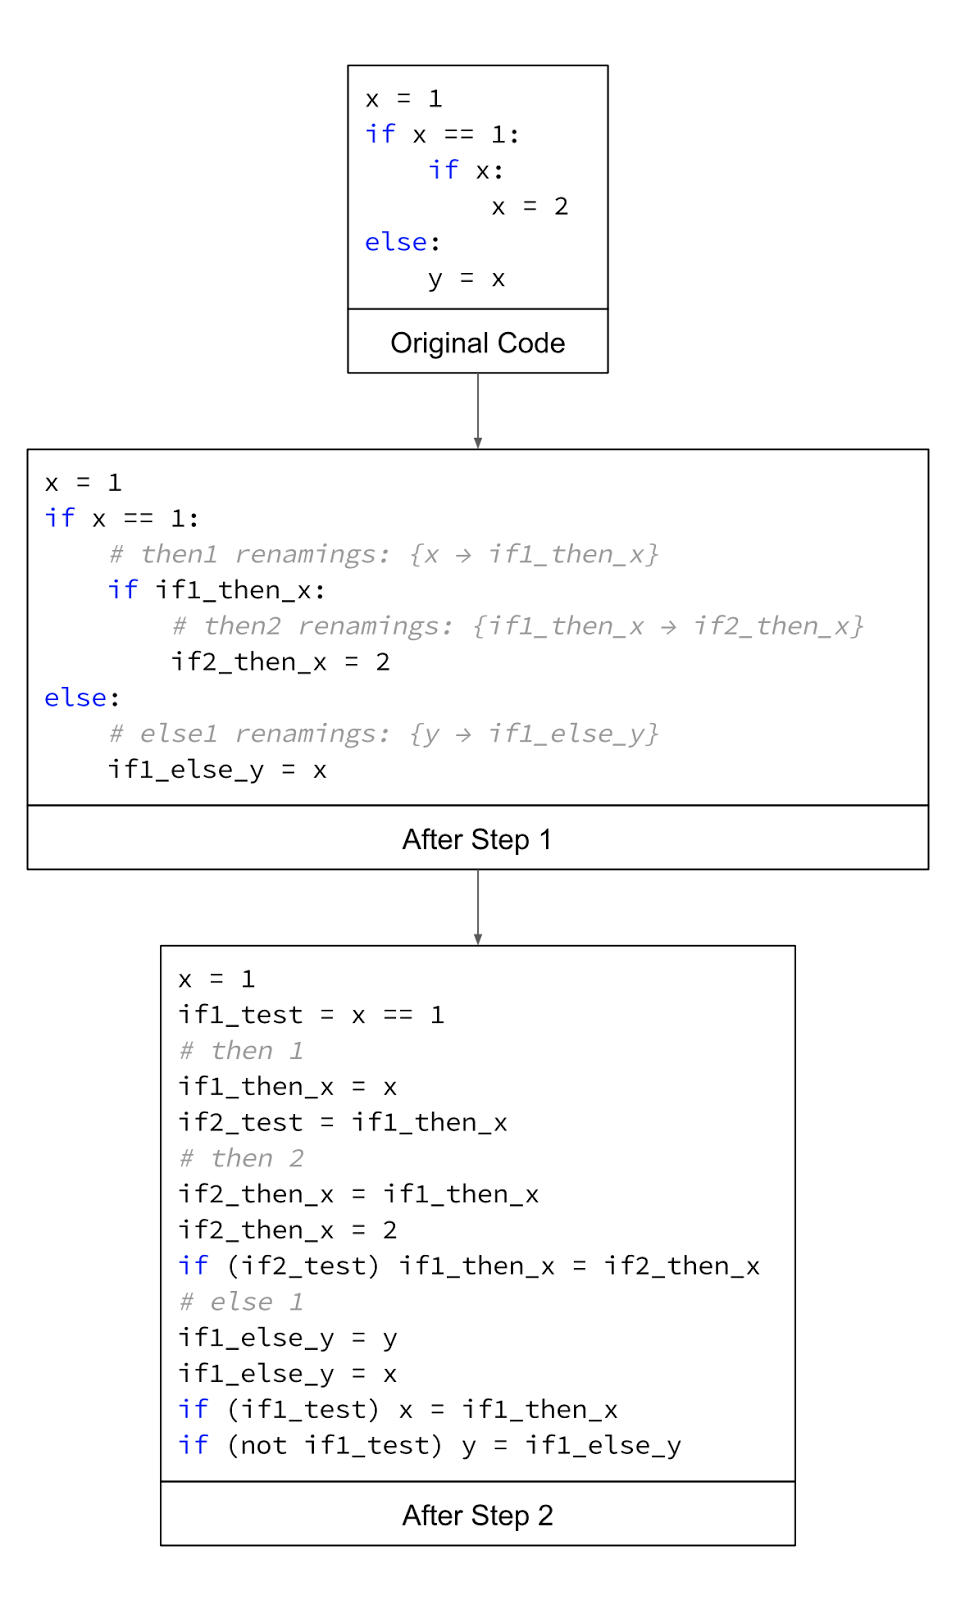
\includegraphics[width=\columnwidth]{cmov_if_transofrmation.png}
\caption{ An example of applying our constant time transformation on the Python program in "Original Code"}
\label{fig:cmov_if_transofrmation}
\end{figure}

Both steps must be performed recursively to nested ifs after being applied to the outer statement. Example of code, generated by this transofrmation may be seen on Figure \ref{fig:cmov_if_transofrmation} Conditional moves are represented by the following pseudo code: \texttt{if (test) dest = src}

\subsection{Cache Side-Channel defense}
Removing conditional control flow results in an almost complete solution to the issue of an attacker knowing what is executing since variables aren’t selectively read or written based on a test condition. The only stumbling block is when the first operand of a conditional move (the source) comes from memory. In that case, the processor only requests the value from the cache if the condition is met. This can be fixed rather easily with some overhead by always reading the left operand, selectively changing it, and always writing it back.

\section{Evaluation}

\begin{figure*}[tp]
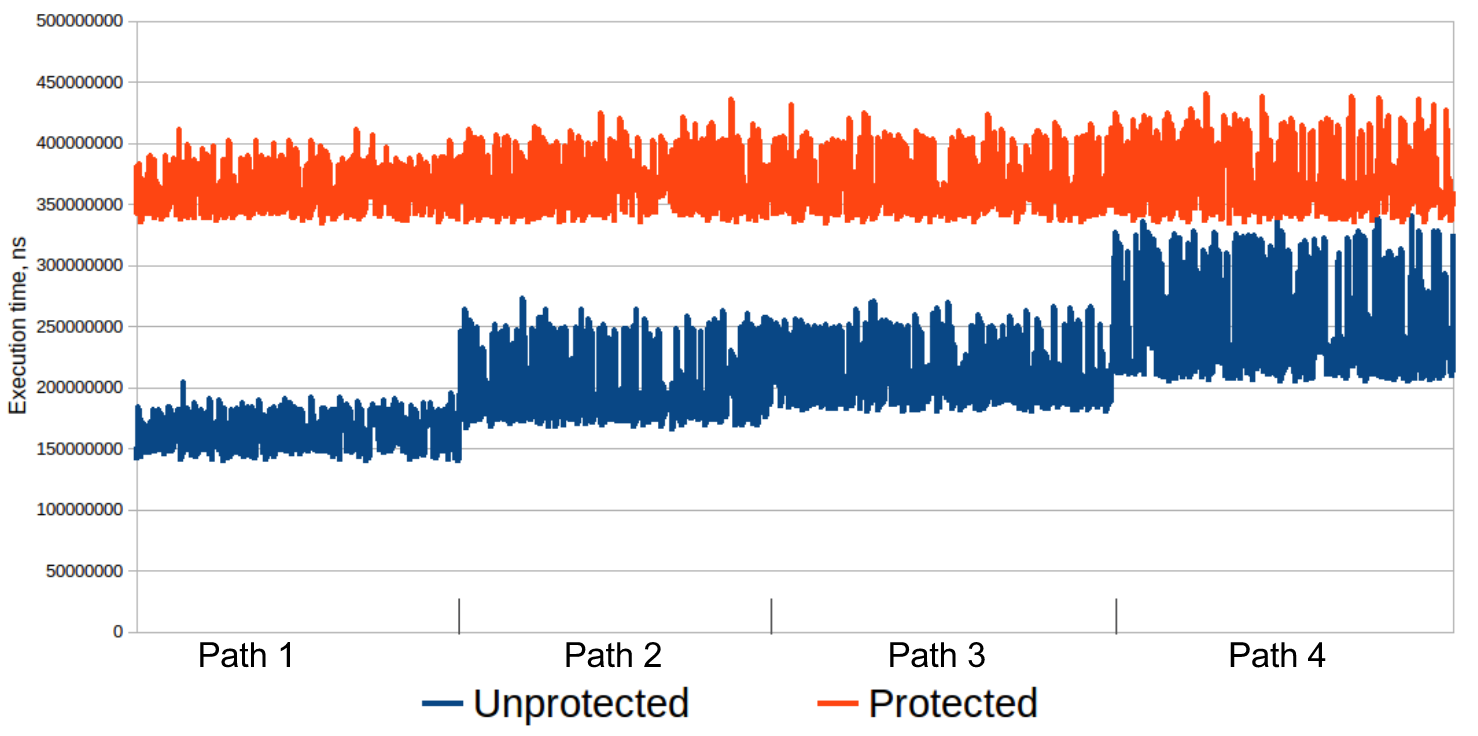
\includegraphics[width=\textwidth]{./timings_protected_vs_unprotected.png}
\caption{Results from timing multiple executions of two binaries, one produced by an insecure compiler (blue) and one by our constant time compiler (red).}
\label{fig:timings}
\end{figure*}

Figure \ref{fig:timings} the security of our compiler, we compiled a program consisting of a loop iterating over two if statements (resulting in 4 possible paths of execution). The program would select the test condition for each if statement randomly on each run, independent of any manual input. The above figure shows runtime in nanoseconds on the y-axis of both the output binary from the unsecured Python compiler in blue and the constant time compiler in red. The timings of both binaries have been sorted into the 4 paths, 1 being no branches taken, 2 and 3 being either the first or second if statement executed, and 4 being both branches taken. With no protections, the path taken is clear after only a few iterations of the program, revealing the secret value that determined the test of each if statement. A notable result here is that paths 2 and 3 differ by only one instruction in length. With enough iterations, even these single instruction differences become evident. When the program was compiled with our constant time transformations, there appears to be no timing differences, even between paths 1 and 4, despite the semantics of the language being completely preserved.\\
Our implementation introduces a non-negligible overhead. On average in the above figure, our solution is 1.76 x slower, compared to Zigzaggers 1.2 x. If timing attacks are a practical concern, then some overhead will be necessary, as an attacker can’t know if the faster or slower computation was performed. However, we still have a 1.4 x slowdown as compared to every path being taken in the unprotected binary (path 4). This is almost entirely due to the excessive safety and naivety of the transformation as defined above. Many renamings and initializations can be removed while preserving the constant time nature of the code, which we do not explore in this work. With optimizations added to the algorithm, runtime should actually be lower than running all branches in the unprotected binary, as we will not run into issues with mispredicted branches and pipeline flushes.

\section{Related Work}
Timing attacks endanger a wide range of secure applications, including ones that do not utilize SGX, especially cryptographic libraries~\cite{arnaud2013timing}~\cite{garcia2016constant} and allow local adversary to recover private key in under 5 minutes~\cite{schwarz2017malware}. For that reason, timing side-channels were studied for over 2 decades~\cite{kocher1996timing} and many defences have been proposed, such as reducing accuracy with noise~\cite{hu1992reducing}, spawning multiple threads to execute all branches~\cite{devriese2010noninterference} or closing access to the clock~\cite{percival2005cache} entirely. Another interesting solution to timing side channel was introduced in FaCT~\cite{cauligi2017fact}---new constant-time, C++ compliant Domain Specific Language---which allows developers to write idiomatic, constant time code, but they do not protect against branch shadowing.\\
Cache side-channel attacks are also applicable in non-SGX case and has been a threat~\cite{osvik2006cache} to cryptographic libraries. There are effective defences against cache-based attacks, including a clever usage of transactional memory~\cite{gruss2017strong}, proposed in 2017.\\
There is a research, dedicated specifically to SGX side-channels, including work done by Lee et al, in which a novel Branch Shadowing attack~\cite{lee2016inferring} was introduced, as well as defences against it in software and hardware.\\
Many defences are focused on a particular side-channel and may not always efficiently stack with each other. Still, there are defences that attempt to protect against a very wide range of attacks, such as Racoon~\cite{rane2015raccoon}, which introduces the notion of Digital Side-Channel---defined as a side-channel that carries information over discrete bits---and defends against them, however protections do not include Branch Shadowing.\\
Verification of constant time implementation is an extensively researched subject. The conventional way to guarantee ground truth on timing is a set of benchmarks, such as one used in to verify fixed-point constant-time math library~\cite{andrysco2015subnormal}. Static analysis at various levels also may be effective: one approach analyzes~\cite{almeida2016verifying} LLVM IR with formalization that reduces the constant-time security of a program P to safety of a product program Q that simulates two executions of P. This work can help ensure that an implementation is constant time.

\section{Conclusion}
Side channels, such as cache and timing leakage, as well as the newly proposed branch shadowing attack, propose dangerous threats to the otherwise secure SGX solution provided by intel. We were able to extend the safety guarantees that can be provided by the compiler beyond Zigzagger’s branch shadowing mitigation, to include both cache and timing side-channel protection. The solution, which renames variables to safely execute both branches of each conditional branch, should be able to be made nearly as fast as the longest execution path of an unsecured program, and has been shown to produce completely constant time binaries. Security sensitive programs, such as cryptographic libraries will see much of their maintenance overhead decrease (due to the ability to write idiomatic code even for constant time implementations) if they adopt compilers that can guarantee their code will always be compiled to a side-channel free binary.


{\bibliographystyle{ACM-Reference-Format}
\bibliography{bibliography}}

\end{document}

